% !TEX root = ../main.tex
\documentclass[../main.tex]{subfiles}

\documentclass{article}
\usepackage{array}
\usepackage{lipsum}

\begin{document}

\section{Anforderungsliste Version 2}

Die nachfolgende Tabelle zeigt die Anforderungsliste des Pfadfinder-Fahrzeugs.

\textbf{Legende} \\ F = Festanforderung \\ M = Mindestanforderung \\ W = Wunschanforderung

\subsection{Allgemeine Anforderungen}

\begin{tabular}{|l|p{0.5cm}|p{4cm}|p{10cm}|}
  \hline
               & \textbf{F} &                      & \textbf{Daten}                                                                                                                                                                                                               \\
  \textbf{Nr.} & \textbf{M} & \textbf{Bezeichnung} & \textbf{Werte}                                                                                                                                                                                                               \\
               & \textbf{W} &                      & \textbf{Erläuterungen}                                                                                                                                                                                                       \\
  \hline
  1.1          & W          & Wettbewerb           & Team 10 wird im Wettbewerb einen Podestplatz erreichen.                                                                                                                                                                      \\
  \hline
  1.2          & F          & Wettbewerbsort       & Voraussichtlich wird der Wettbewerb im Foyer der Mensa HSLU Technik und Architektur in Horw durchgeführt.                                                                                                                    \\
  \hline
  1.3          & F          & Projektabgabe        & Der PREN 1 Schlussbericht ist bis zum 10. Januar 2025 abzugeben.                                                                                                                                                             \\
  \hline
  1.4          & F          & Eigenkonstruktion    & Einzelne Systemkomponenten wie z.B. Räder, Servos, Motoren, Mikrocontroller, Kamera, etc. dürfen zugekauft und eingesetzt werden. Das zu realisierende Fahrzeug als Ganzes muss jedoch zwingend eine Eigenkonstruktion sein. \\
  \hline
  1.5          & F          & Software             & Es dürfen Software-Komponenten und Software-Services von Fremd-Herstellern verwendet werden.                                                                                                                                 \\
  \hline
  1.6          & F          & Eingriffe            & Ein Eingreifen auf das Fahrzeug ist nach dem Start nicht mehr erlaubt.                                                                                                                                                       \\
  \hline
  1.7          & F          & Sicherheit           & Das Team ist während sämtlichen Betriebs- und Test-Phasen verantwortlich für die Sicherheit des Fahrzeuges und den Schutz der Personen.                                                                                      \\
  \hline
  1.8          & W          & Nachhaltigkeit       & Erfüllt Anforderungen nach SDG 12. Insbesondere die Unterziele 12.4 und 12.5.                                                                                                                                                \\
  \hline
  1.9          & W          & Materialien Mechanik & Mechanikkonstruktionen vorzüglich Materialien.                                                                                                                                                                               \\
  \hline
  1.10         & W          & Lieferwege           & Wenn möglich Materialien und Kaufteile aus Europäischen Lagern beziehen.                                                                                                                                                     \\                                                                                                               \\
  \hline
\end{tabular}

\subsection{Gerät}
\begin{tabular}{|l|p{0.5cm}|p{4cm}|p{10cm}|}
  \hline
               & \textbf{F}            &                                                                       & \textbf{Daten}                                                                                                                                                                                                                                                                                                                             \\
  \textbf{Nr.} & \textbf{M}            & \textbf{Bezeichnung}                                                  & \textbf{Werte}                                                                                                                                                                                                                                                                                                                             \\
               & \textbf{W}            &                                                                       & \textbf{Erläuterungen}                                                                                                                                                                                                                                                                                                                     \\
  \hline
  2.1          & F                     & Autonomität                                                           & Das Fahrzeug muss den vorgegebenen Parcours von Start bis Ziel ohne Zugriff von aussen absolvieren können.                                                                                                                                                                                                                                  \\
  \hline
  2.2          & F                     & Hardwarekomponenten                                                   & Alle zum Betrieb benötigten Hardware-Komponenten wie z.B. Sensoren, Aktoren, Steuergeräte, Kamera, etc. müssen sich im oder auf dem Fahrzeug befinden.                                                                                                                                                                                     \\                                                                                                                                                                                                                                                                                                                                           \\
  \hline
  2.3          & F Softwarekomponenten & Alle Berechnungen und Software muss auf dem Roboter betrieben werden.                                                                                                                                                                                                                                                                                                                                              \\
  \hline
  2.4          & M                     & Betriebsbereitschaft                                                  & Das Fahrzeug muss innerhalb von maximal einer Minute im Startbereich manuell platziert und aufgebaut werden, sowie betriebsbereit sein.                                                                                                                                                                                                    \\
  \hline
  2.5          & W                     & Gesperrte Wegpunkte                                                   & Die gesperrten Wegpunkte sollten vom Fahrzeug erkannt werden.                                                                                                                                                                                                                                                                              \\
  \hline
  2.6          & W                     & Hindernis auf Strecke                                                 & Mögliche Hindernisse sollten vom Fahrzeug erkannt werden.                                                                                                                                                                                                                                                                                  \\
  \hline
  2.7          & F                     & Hindernisbewältigung                                                  & Befährt das Fahrzeug eine Strecke mit einem Hindernis, so muss dieses erkannt und aktiv von der Strecke aufgenommen werden. Sobald das Fahrzeug die besagte Stelle passiert hat, muss das Hindernis wieder an die Ursprungsposition zurückgestellt werden. Die Toleranzzone beim Zurückstellen des Hindernisses beträgt 20 mm (umlaufend). \\
  \hline
  2.8          & F                     & Auswahl Zielposition                                                  & Die Zielposition (1, 2 oder 3) muss am Fahrzeug mittels einem Wahlschalter ausgewählt werden können.                                                                                                                                                                                                                                       \\
  \hline
  2.9          & F                     & Startbefehl                                                           & Der Startbefehl wird mittels einem Schalter oder Taster am Fahrzeug erteilt. Gleichzeitig wird die Sicht auf die Strecke freigegeben und die Zeitmessung gestartet.                                                                                                                                                                        \\
  \hline
  2.10         & F                     & Leitlinien                                                            & Das Fahrzeug muss sich während des gesamten Parcours auf den vorgegebenen Leitlinien bewegen.                                                                                                                                                                                                                                              \\
  \hline
  2.11         & F                     & Not-Aus                                                               & Das Fahrzeug muss über einen leicht zugänglichen Not-Aus-Knopf oder -Schalter verfügen, der alle mechanisch-dynamischen Prozesse sofort unterbricht.                                                                                                                                                                                       \\
  \hline
  2.12         & F                     & Gewicht                                                               & Das Fahrzeug darf das Maximalgewicht von 2 kg nicht überschreiten.                                                                                                                                                                                                                                                                         \\
  \hline
  2.13         & W                     & Schutzklasse                                                          & Mindestens IP-10 sollte gewährleistet sein.                                                                                                                                                                                                                                                                                                \\
  \hline
  \multicolumn{4}{|p{\dimexpr1.5cm+3cm+6cm+1.5cm}|}{Die letzte Zeile dieser Tabelle soll über die volle Seitenbreite gehen und flexibel gefüllt werden.}                                                                                                                                                                                                                                                                                                    \\
  \hline
\end{tabular}

\newpage

\begin{tabular}{|l|p{0.5cm}|p{4cm}|p{10cm}|}
  \hline
               & \textbf{F} &                           & \textbf{Daten}                                                                                                                                                                                                              \\
  \textbf{Nr.} & \textbf{M} & \textbf{Bezeichnung}      & \textbf{Werte}                                                                                                                                                                                                              \\
               & \textbf{W} &                           & \textbf{Erläuterungen}                                                                                                                                                                                                      \\
  \hline
  2.14         & F          & Dimensionen               & Das Fahrzeug darf die Dimensionen 30$\times$30 cm zu jeder Zeit, ausser beim Bewegen von Hindernissen, nicht überschreiten. Zudem ist die Höhe des Fahrzeugs (oder allfälliger Anbauteile) auf maximal 80 cm beschränkt.    \\
  \hline
  2.15         & F          & Zielposition              & Das Erreichen der Zielposition muss vom Fahrzeug in einer passenden Form visuell oder akustisch angezeigt werden. Zudem muss das Fahrzeug innerhalb eines Kreises von 30 cm Durchmesser um den Zielpunkt zum Stehen kommen. \\
  \hline
  2.16         & W          & Energieversorgung         & Die Energieversorgung soll mit einem Akku realisiert werden, der über eine physische, steckbare Schnittstelle innerhalb von 6h wieder aufgeladen werden kann.                                                               \\
  \hline
  2.17         & W          & Akkulaufzeit              & Im aktiven Betrieb des Fahrzeugs soll eine Akkulaufzeit von mindestens 25 Minuten gewährleistet sein.                                                                                                                       \\
  \hline
  2.18         & W          & Debug-Schnittstelle       & Die Elektronik des Fahrzeugs soll über eine Debug-Schnittstelle verfügen, die es ermöglicht, aktuelle Zustände und Signale auszulesen.                                                                                      \\
  \hline
  2.19         & W          & Controlling-Schnittstelle & Die Elektronik des Fahrzeugs soll über Schnittstelle verfügen, über welche die Aktoren aktiv angesteuert werden können.                                                                                                     \\
  \hline
  2.20         & W          & Zeitmessung               & Das Gerät bietet die Möglichkeit die verstrichene Zeit seit Start anzugeben. Diese Zeitmessung wird optisch oder über eine Programmschnittstelle an das Team weitergegeben.                                                 \\
\end{tabular}

\subsection{Parcours}
\begin{tabular}{|l|p{0.5cm}|p{4cm}|p{10cm}|}
  \hline
               & \textbf{F} &                               & \textbf{Daten}                                                                                                                                                                                                       \\
  \textbf{Nr.} & \textbf{M} & \textbf{Bezeichnung}          & \textbf{Werte}                                                                                                                                                                                                       \\
               & \textbf{W} &                               & \textbf{Erläuterungen}                                                                                                                                                                                               \\
  \hline
  3.1          & F          & Wege-Netzwerk                 & Das Graph-Topologie und der Startknoten sind bekannt. (Abbildung~\ref{fig:wege-netzwerk})                                                                                                                            \\
  \hline
  3.2          & F          & Zielpunkte                    & Die möglichen Zielpunkte sind bekannt, doch der definitive Zielpunkt wird erst unmittelbar vor dem Start des Parcours von der Juri bekannt gegeben und ist vorher nicht bekannt. (Abbildung~\ref{fig:wege-netzwerk}) \\
  \hline
  3.3          & F          & Wegpunkte                     & Insgesamt gibt es acht Wegpunkte. Die Wegpunkte sind aufgeklebte Vollkreise (weiss) mit einem Durchmesser von 7 bis 12 cm. (Abbildung~\ref{fig:wegpunkt})                                                            \\
  \hline
  3.4          & F          & Untergrund                    & Der Untergrund entspricht dem Bodenbelag des Foyers der Mensa auf dem Campus der Hochschule Luzern für Technik und Architektur in Horw. (Abbildung~\ref{fig:fliesenboden})                                           \\
  \hline
  3.5          & F          & Leitlinien                    & Die Wegpunkte sind mit hellen Leitlinien (aufgeklebtes Klebeband) verbunden. Die Breite der Leitlinien beträgt ca. 20 mm.                                                                                            \\
  \hline
  3.6          & F          & Abmessungen                   & Der Abstand der Wegpunkte ist variabel zwischen 0.5 bis 2.0 m. Die Gesamtfläche des Wege-Netzwerkes beträgt ca. 4.5 x 4.5 m.                                                                                         \\
  \hline
  3.7          & F          & Gesperrte Wegpunkte           & Die gesperrten Wegpunkte dürfen nicht befahren werden. Sie sind bis zum Start unbekannt und mittels einem Leitkegel gekennzeichnet.                                                                                  \\
  \hline
  3.8          & F          & Hindernis auf Strecke         & Die Strecke darf befahren werden, doch das Hindernis muss aktiv von der Strecke aufgenommen und am gleichen Ort wieder zurückgestellt werden.                                                                        \\
  \hline
  3.9          & F          & Nicht vorhandene Teilstrecken & Leitlinien können aus dem Wege-Netzwerk entfernt werden. Die entsprechenden Verbindungen können nicht befahren werden.                                                                                               \\
  \hline
  3.10         & F          & Streckenbedingungen           & Die Streckenbedingungen (Sperrung, Hindernisse, nicht vorhandene Teilstrecke) sind bis zum Start unbekannt.                                                                                                          \\
  \hline
  3.11         & F          & Startbereich                  & Die Grösse des Startbereichs beträgt 30 x 30 cm. Das Fahrzeug darf diese Dimensionen nicht überschreiten.                                                                                                            \\
  \hline
  3.12         & F          & Start                         & Sobald die Sicht auf die Strecke freigegeben wird, beginnt ebenfalls die Zeitmessung.                                                                                                                                \\
  \hline
  3.13         & M          & Parcours-Laufzeit             & Die Laufzeit von Start bis Ziel darf maximal vier Minuten betragen. Wird das Ziel innert vier Minuten nicht erreicht, ist der Lauf ungültig.                                                                         \\
  \hline
\end{tabular}

\subsection{Simulation}
\begin{tabular}{|l|p{0.5cm}|p{4cm}|p{10cm}|}
  \hline
               & \textbf{F} &                           & \textbf{Daten}                                                                                                                                                                                     \\
  \textbf{Nr.} & \textbf{M} & \textbf{Bezeichnung}      & \textbf{Werte}                                                                                                                                                                                     \\
               & \textbf{W} &                           & \textbf{Erläuterungen}                                                                                                                                                                             \\
  \hline
  4.1          & F          & Betriebssystem            & Die Simulation muss auf Windows ausführbar sein.                                                                                                                                                   \\
  \hline
  4.2          & W          & Betriebssystem            & Die Simulation soll auf Linux und auch Windows ausführbar sein.                                                                                                                                    \\
  \hline
  4.3          & W          & Benutzeroberfläche        & Den Wegstrecken und Netzwerkknoten können beliebige Streckenereignisse zugewiesen werden.                                                                                                          \\
  \hline
  4.4          & M          & Darstellung               & Die Simulation muss 2-dimensional dargestellt werden.                                                                                                                                              \\
  \hline
  4.5          & W          & Darstellung               & Die Simulation kann 3-dimensional dargestellt werden.                                                                                                                                              \\
  \hline
  4.6          & W          & Pfadfindungsalgorithmen   & In der Simulation sollen verschiedene Pfadfindungs-algorithmen (z.B. Dijkstra, A*-Algorithmus, etc.) implementiert werden für eine direkte Gegenüberstellung in Zuverlässigkeit und Schnelligkeit. \\
  \hline
  4.7          & W          & Zeitauswertung            & In der Simulation soll eine approximierte Zeitauswertung, basierend auf heuristischen Abschätzungen, möglich sein.                                                                                 \\
  \hline
  4.8          & W          & Visualisierung des Pfades & Der vorgeplante Pfad soll währrend der Simulation angezeigt werden, um das Verhalten des Fahrzeugs besser nachvollziehen zu können.                                                                \\
  \hline
  4.9          & W          & Hindernistypen            & Verschiedene Arten von Hindernissen (beweglich und stationär) sollen simuliert werden können.                                                                                                      \\
  \hline
  4.10         & W          & Fahrzeugparameter         & Fahrzeugparameter (Geschwindigkeit, Wendekreis, Sensorreichweite, etc.) sollen editierbar sein.                                                                                                    \\
  \hline
  4.11         & W          & Datenexport               & Die Daten, welche während der Simulation generiert werden, sollen exportierbar sein.                                                                                                               \\
  \hline
  4.12         & W          & Error-Handling            & Der Simulator muss robust auf Fehler reagieren und darf keinesfalls abstürzen. Zudem sollen Fehlerzustände abgefangen und klar dokumentiert werden.                                                \\
  \hline
\end{tabular}

\subsection{Herstellungsressourcen}
\begin{tabular}{|l|p{0.5cm}|p{4cm}|p{10cm}|}
  \hline
               & \textbf{F} &                                  & \textbf{Daten}                                                                                                                                                                                                                                                                                                                                                                                \\
  \textbf{Nr.} & \textbf{M} & \textbf{Bezeichnung}             & \textbf{Werte}                                                                                                                                                                                                                                                                                                                                                                                \\
               & \textbf{W} &                                  & \textbf{Erläuterungen}                                                                                                                                                                                                                                                                                                                                                                        \\
  \hline
  5.1          & W          & Materialbeschaffung              & Materialien und Komponenten sollen vorzugsweise von folgenden Lieferanten bestellt werden: \newline - Conrad Electronic \newline - Distrelec \newline - Mädler \newline - Farnell                                                                                                                                                                                                             \\
  \hline
  5.2          & F          & Budget                           & Für die Realisierung des Projekts stehen dem Team insgesamt 500 CHF zur Verfügung. Davon dürfen maximal 200 CHF in PREN 1 ausgegeben werden.                                                                                                                                                                                                                                                  \\
  \hline
  5.3          & F          & Normteile ab HSLU Lagerbestand   & Normteile (Schrauben, Lager, Rohmaterial, Widerstände, Kondensatoren, etc.) aus dem HSLU Lagerbestand dürfen kostenlos verwendet werden.                                                                                                                                                                                                                                                      \\
  \hline
  5.4          & F          & Persönlicher 3D-Drucker          & Wird für das Projekt ein persönlicher 3D-Drucker verwendet, so muss die verarbeitete Menge ausgewiesen werden.                                                                                                                                                                                                                                                                                \\
  \hline
  5.5          & F          & Herstellungs-ressourcen der HSLU & Dem Team stehen für die Umsetzung des Projekts (PREN 1 und PREN 2) die folgenden Ressourcen der HSLU zur Verfügung: \newline - maximal 25 h Maschinenlaufzeit der 3D-Drucker \newline - maximal 1 h Maschinenlaufzeit des Lasergeräts \newline - maximal 10 Arbeitsstunden des Werkstattpersonals Elektrotechnik \newline - maximal 10 Arbeitsstunden des Werkstattpersonals Maschinentechnik \\
  \hline
\end{tabular}

\newpage

\subsection{Abbildungen}
Folgend sind sämtliche Abbildungen aufgeführt, auf die in der Anforderungsliste
referenziert wurde.

\begin{figure} [ht]
  \centering
  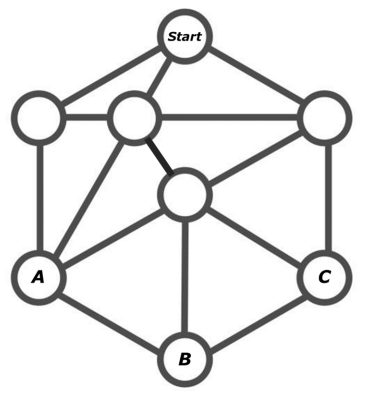
\includegraphics[scale=0.5]{../resources/WegeNetzwerk.png}
  \caption{Vorgegebenes Wege-Netzwerk mit Start- und Zielpositionen A-B-C}
  \label{fig:wege-netzwerk}
\end{figure}

\begin{figure} [ht]
  \centering
  
\includegraphics[scale=0.5]{../resources/Wegpunkt.png}
  \caption{Typischer aufgeklebter Wegpunkt}
  \label{fig:wegpunkt}
\end{figure}

\begin{figure} [ht]
  \centering
  
\includegraphics[scale=0.05]{../resources/Fliesenboden.jpg}
  \caption{Fliesenboden im Foyer der Mensa}
  \label{fig:fliesenboden}
\end{figure}

\newpage

\end{document}
